\documentclass[11pt]{article}

\usepackage{amssymb}
\usepackage[english]{babel}
\usepackage{changepage}
\usepackage{cite}
\usepackage{float}
\usepackage[margin=1.5in]{geometry}
\usepackage{graphicx}
\usepackage{lmodern}
\usepackage{setspace}
\usepackage{tabularx}
\usepackage{booktabs}
\usepackage[table,xcdraw]{xcolor}
\usepackage{adjustbox}
\usepackage{url}
\usepackage{listings}
\usepackage{appendix}

\usepackage{tikz}
\usetikzlibrary{shapes.geometric, arrows}
\usepackage{standalone}

\usepackage[T1]{fontenc}

\bibliographystyle{ieeetr}

\graphicspath{{figures}}

\lstset{
    basicstyle=\small,
    showspaces=false,
    showstringspaces=false,
    tabsize=2,
    title=\lstname,
}

\onehalfspacing

\begin{document}
\thispagestyle{empty}
\begin{center}
\begin{Large}
\emph{Thesis Submitted for Master of Science in Computer Science} \\
Department of Computer Science \\
Rochester Institute of Technology \\
\end{Large}
\vspace{4em}
{\huge Generalized Model of Cognitive Workload} \\
\vspace{3em}
{\LARGE Taylor Carpenter} \\
{\tt tjc1575@rit.edu} \\
\vspace{3em}
\begin{adjustwidth}{.5in}{.5in}
Chair: Dr. Zack Butler \hfill {\tt zjb@cs.rit.edu} \\
\vspace{2em}
\hrulefill \\
\vspace{3em}
Reader: Dr. Esa Rantanen \hfill {\tt emrgsh@rit.edu} \\
\vspace{2em}
\hrulefill \\
\vspace{3em}
Observer: Sean Strout \hfill {\tt sps@cs.rit.edu} \\
\vspace{2em}
\hrulefill
\end{adjustwidth}
\vspace{2em}
Rochester, NY 14623 USA \\
\vspace{2em}
\today
\end{center}
\pagebreak
\thispagestyle{empty}
\begin{center}
\begin{large}
A Thesis Submitted\\
in\\
Partial Fulfillment of the\\
Requirements for the Degree of\\
Master of Science in Computer Science

\vspace{.5in}

Department of Computer Science\\
B. Thomas Golisano College of Computing and Information Sciences\\
Rochester Institute of Technology\\
Rochester, NY 14623 USA
\end{large}
\end{center}
\pagebreak
\thispagestyle{empty}
\begin{abstract}
\emph{Author remarks are made in italics. Bolded sections signify passages that I am particiularly concerned about.}
\end{abstract}
\clearpage
\pagenumbering{arabic}
\tableofcontents
\listoffigures
\listoftables
\pagebreak

\section{Introduction}
% General introduction stuff
% What is the research area?	

\section{Background}
	\subsection{Terminology}
	The following subsections layout the definitions that are used for various terminology that appears throughout this research. Some of the terms are commonly used in this area of research but have various meanings depending on the field and background from which the research originates. Other terms are being assigned unique meaning for the purposes of this research. For the sake of clarity, the major terms are explained explicitly, ideally removing confusion on how the terms are being used.
	
		\subsubsection{Cognitive Workload}
		Many definitions exist for cognitive workload, as it is a theoretical concept that is intuitive to understand but difficult to fully encapsulate within a single statement. For the purposes of this research, the definition of cognitive workload is that proposed by Meshkati: ``mental workload [is] a multidimensional construct that reflects the interaction of such elements as task and system demands, operator processing capabilities and effort, subjective performance criteria, operator information processing behavior and strategies, and finally, operator training and prior experience''~\cite{Meshkati}. Since cognitive workload is a theoretical construct that exists in the mind, there are no methods of measuring the load directly. Instead, loading tasks can be used to affect workload while measurements, such as various psychophysiological readings, can be examined that allow for inferences to be made about cognitive workload.  With respect to this research, descriptions about measuring cognitive workload are in fact referring to the indirect measurement of factors affected by workload and making inferences about the underlying load. Another term commonly used in this line of research is ``operator function state'' or OFS. The definition of OFS used in this study is that put forth by Hockey: ``the variable capacity of the human operator for effective performance in response to task and environmental demands, and under the constraints imposed by cognitive and physiological processes that control and energize behavior''~\cite{Hockey}. In many applications, such as the current research and various other similar studies, cognitive workload and OFS can be seen as the same construct and used interchangeably. For the sake of clarity, cognitive workload is the term that is used throughout this research, although studies that are referenced herein may use the term OFS.
		
		\subsubsection{Study}
		Study, for the purposes of this research, refers to the data collection process that involved the help of participants. The end result of the study was the production of psychophysiological data that was then processed and analyzed as part of the remaining research.  When being used in reference to the work of other researches, however, study refers to the entire research process as reported in the cited writings.
		
		\subsubsection{System}
		In this research, system refers to the processes and Python scripts that acted on the data collected from the study. This includes everything from the preprocessing of sensor data to the training and evaluation of classification models. 		
		
		\subsubsection{Model / Classifier}
		Another term that is used throughout this research is ``model''. In this case, the more mathematical definition of model that is used in the context of machine learning is intended, rather than a strictly psychological definition. A model, as used in machine learning, is a system that can take in input data and produce some output as defined by patterns present in historical data. This system may be a black-box, which cannot be defined or explained effectively by a person, or it may be described with well defined rules, depending on the technique used. Since the current research deals with the classification of data, the term classifier is also used to refer to the model. It should be noted that ``classifier'', which is the trained model, is distinct from ``classification method'', which is the particular format of the model, such as artificial neural network.
	% Cognitive Workload
	% "Study"
	% "System"
	% "Model"
	
	\subsection{Cognitive Workload}
	% What is it?
	% Current / previous research into workload

	\subsection{Physiological Measures}
	% What measures have been used in this line of research?
		% EEG
		% HR
		% Eye movement
		% Respiration
		% Cranial blood flow
	% When did EEG start being used as a measure of workload?
	% What does EEG show?
	
	\subsection{Random Forest}
	% What is it?
	% Who first created it?
	% Why are ensemble methods useful?
	% What can be tuned?
	% Pros / Cons
	
	\subsection{Artificial Neural Network}
	% What is it?
	% Who first created it?
	% What can be tuned?
	% Pros / Cons

\section{Related Work}
Classifying cognitive workload has been the subject of many studies. The majority of studies have dealt with creating an individual model unique to each participant, with the study consisting of only one task. These studies commonly use EEG and heart rate as psychophysiological features~\cite{Wang_R, Zhang, Wilson, Yang}. While EEG data is consistently used in cognitive workload studies, the subsequent features generated from the data vary. Some of studies, such as the work performed by Wilson et al.~\cite{Wilson}, use log power spectrum information from the EEG measurements while other studies, such as that by Zhang et al.~\cite{Zhang}, use combinations of EEG power spectrum information, called task load indices. In addition to EEG and heart rate, some studies include blink rate~\cite{Wilson, Wilson_2002} and respiration rate~\cite{Wilson_2003} as features. Other studies used blinking and eye movement measures to correct artifacts in EEG data~\cite{Wang_R}. The general layout for each of the studies was roughly the same; participants were attached to a variety of sensors and then asked to perform a loading task at varying difficulty levels to induce different cognitive workloads. The two most common loading tasks used were MATB~\cite{Estepp} and AutoCAMS~\cite{Lorenz}. These systems are commonly used due to their ability to systematically vary the difficulty settings. 

A variety of different classifiers have been used in studies in an attempt to model cognitive workload. The study covered by Yang et al.~\cite{Yang} uses a system of fuzzy inference rules to perform realtime classification of cognitive workload for the purposes of adaptive automation triggering. An SVM Regressor was used by Ke et al.~\cite{Ke} to produce a cognitive workload index, a particular number corresponding to cognitive workload level. Another study~\cite{Wang_R} explored the use of an Adaptive-Network-based Fuzzy Inference System that was trained using differential evolution and ant colony search as a means of predicting levels of cognitive workload. Fuzzy C-Means clustering was used in a study~\cite{Zhang} as a means of classification through clustering. The study completed by Wilson et al.~\cite{Wilson} used an artificial neural network. All of these studies have shown adequate results but have failed to address the larger scope of generalizability. One study~\cite{Wang_Z} used a bayesian model to explore the ability of a model to be used on multiple subjects, learning from and tested on a dataset consisting of data from multiple participants. What the study lacked, however, was the ability to handle novel data; that is, classify on a participant that was previously unseen. A different study~\cite{Ke} falls in a similar category, however it deals with multiple tasks rather than multiple participants. The study involved testing on data from an unseen task,  showing the possibility for full generalization. An additional study~\cite{Christensen} demonstrated how cognitive workload metrics for a single individual can vary substantially across multiple days. This adds an additional challenge to generalizability as the model not only has to account for different subjects and tasks, but also the variation within subjects across multiple days.


\section{Problem Statement}
While many studies have focused on individualized models of cognitive workload using machine learning, few studies have produced results that are of use outside of a controlled lab setting. In a practical application, the training of a model to each individual for every task they may perform would be far too time consuming and costly. This research investigates the effectiveness of a generalized model of cognitive workload based on psychophysiological measures. In order for the model to be generalized, it should be robust against differences between individuals and between the tasks being performed. It should also be effective at handling novel individuals and tasks. Such a model may or may not be reasonably developed due to the complexity of the human mind. Ideally the resulting model could be used outside of a controlled setting with automatic data processing and realtime classification.

A driving factor behind this work is usability in a real-world setting. As such, design decisions were made that favor low-cost, easy-to-use sensors with little to no empirical cleaning of data. The models were trained using the machine learning techniques of artificial neural networks and random forests and tested in a variety of configurations to determine their effectiveness. As is common in this type of study, data for experimentation was collected with sensors from subjects as they participated in cognitive loading tasks of varying difficulties. While no methods used would inhibit realtime analysis, the system focused on offline data.  In the end, this research hopes to address the following hypothesis: a generalized model of cognitive workload can be trained using methods suitable for real-time classification without manual data processing that is more effective than random.
% How is this research different than existing research
% What is the hypothesis that we are trying to solve?
	\subsection{Applications}
	% Why is this research important?
	
		\subsubsection{Adaptive Automation}
		% What is adaptive automation?
		% How does a workload classifier interact with AA?
		% Maintain ideal level of interaction between system and human
		% Why is high workload bad?
		% Why is low workload bad?
		% Existing research related to adaptive automation ( both from my previous class and from the other OFS detector work )
		
		\subsubsection{Research}
		% Some tasks are easier to control workload than others
		% Can increase understanding of difficult to control tasks
		
		%Currently analagous systems are used but are not always predictive
			% Reference 'Workload Transition' for potential issues about cross-domain analysis

\section{Study}
A study was conducted in order to generate and collect the data needed to train the appropriate models. While some previous research~\cite{Wang_Z} has relied on the use of established and validated data collected from other experiments~\cite{Wilson_2010}, the amount of data required to adequately train artificial neural networks was not available. Consequently, a new study was required to generate the large amount of data that was necessary. The study consisted of two tasks, each with a leading baseline trial and three load conditions. The load condition trials were ten minutes long and the baseline trials were five minutes long. 
The initial design of the study specified fifteen minute long trials but feedback from the pilot group suggested that at fifteen minutes, task fatigue started affecting performance.

%% Transition?

The study began with a total of ten college-aged participants, similar to existing works~\cite{Ting,Wang_R,Wilson_2010, Yin, Zhang}, however, due to complications, only seven participants completed the entire process. 
Two of the removed participants were excluded due to misfitting of the EEG headset as well as discrepancies between the task difficulties reported versus the average difficulties reported by the other participants. The last removed participant was excluded due to personal issues preventing the completion of the study.

Of the seven participants that completed the study, the ages ranged from 18 to 23 years old, with an average age of 21.1 years. The gender ratio was balanced with three males and four females. Participants lacked any uncorrected hearing or visual impairments that would affect performance on the tasks of the study. 
The following subsections describe each of the tasks as well as the overall layout of the study in its entirety.
	
	\subsection{Multi-Attribute Task Battery (MATB)}
	The first loading task presented to participants was the Multi-Attribute Task Battery (MATB), a task loading system originally developed by NASA~\cite{Comstock}. MATB is a system that has been used in a variety of studies as a means of task loading for the collection of psychophysiological data~\cite{Wilson, Smith, Wang_Z}. The system consists of a multitude of subtasks arranged in such a way as to simulate the tasks a pilot might be required to perform during flight. The particular version of the system used in this study was AF-MATB, an updated version of the original software~\cite{Estepp}. This version is very similar to the original with the majority of the changes affecting how it runs on modern operating systems and adding different options for subtask automation. All of the subtasks of MATB were used in the study, while the scheduling view that shows upcoming events was disabled. Input to the system was in the form of joystick and either keyboard or mouse. Participants were free to decide whether to use the keyboard, mouse, or a combination of the two with the right hand while the joystick was controlled with the left hand. In Figure~\ref{fig:matb}, the main view of MATB with which participants interacted is shown. This includes resource management, systems monitoring, communications, and tracking. 
	
	\begin{figure}[]
	\centering
	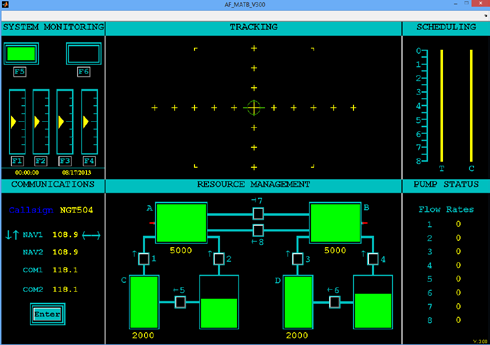
\includegraphics[width=\linewidth]{figures/matb.png}
	\caption[Multi-Attribute Task Battery (MATB) Main View]{Main view of the MATB simulation software. }
	\label{fig:matb}
	\end{figure}
	
	The resource management subtask involved maintaining the amount of fuel that was present in two main tanks within a small acceptable range. Secondary tanks were present and could be used to temporarily store fuel. The participant was required to toggle pumps, controlling the flow of fuel between the tanks. Throughout the trial, pumps would temporarily break, or silently shut-off, preventing the flow of fuel through the pump. The number and frequency of these occurrences depended on the difficulty condition of the trial.
	
	The systems monitoring subtask were centered around two buttons and four gauges. One button was to be kept on while the other button was to be kept off. Throughout the simulation, the buttons changed states and the participant was required to click on the button indicator, or press a corresponding key, to revert the button to the correct state. Colors were used to indicate the state of the buttons. Background color indicated that the button was off, while either red, for the ``off'' button, or green, for the ``on'' button, was used to indicate on. The gauges presented had sliders that would vary in vertical position throughout the simulation. Occasionally, depending on the difficulty condition, a slider would move outside the acceptable range for the gauge and require interaction from the participant, either through a mouse click or key press, to reset the gauge. If an out-of-state system component was not addressed within the response time period of ten seconds, the component was automatically reset to its defaults, within-range state.
	
	The communication subtask required the use of sound. The participant was assigned a particular aircraft callsign. For the duration of the trial, the participant was required to listen to their callsign and respond to the instructions. The communication window included four different communication channels, each set to a particular frequency. Throughout the simulation, recorded audio tracks would play, addressing a particular callsign to change a channel to a desired frequency. If the callsign matched that of the participant, they were to change the specified communication channel to the appropriate frequency using either the mouse or the arrow keys. If the callsign did not match that of the participant, the request was to be ignored. The number and rate of true- and false-alarm requests depended on the difficulty condition of the trial.
	
	The tracking subtask was the only one that required the use of the joystick. The participant simulated steering a plane by keeping a reticle within the acceptable parameters of the tracking window. The amount of drift affecting the reticle and the amount of control the joystick emitted onto the reticle varied throughout the simulation in accordance with the difficulty condition of the trial. 
	
	\begin{table}[]
	\centering
	\adjustbox{max width=\textwidth}{
	\begin{tabular}{llllllll}
	\toprule
	\rowcolor[HTML]{FFFFFF} 
	 &  & \multicolumn{2}{c}{\cellcolor[HTML]{FFFFFF}Communication} & \multicolumn{2}{c}{\cellcolor[HTML]{FFFFFF}System} & \multicolumn{2}{c}{\cellcolor[HTML]{FFFFFF}Resources} \\ \cmidrule(l){3-8} 
	\rowcolor[HTML]{FFFFFF} 
	Load Condition & Tracking & Target & Distractor & Lights & Gauges & Failures & Shut-offs \\ \midrule
	\rowcolor[HTML]{EFEFEF} 
	Low & Low & 6 & 2 & 48 & 42 & 4 & 2 \\
	\rowcolor[HTML]{FFFFFF} 
	Moderate & Moderate & 18 & 10 & 96 & 102 & 20 & 10 \\
	\rowcolor[HTML]{EFEFEF} 
	High & High & 30 & 12 & 110 & 120 & 40 & 20 \\ \bottomrule
	\end{tabular}
	}
	\caption[Multi-Attribute Task Battery (MATB) Load Condition Parameters]{The parameter values specifying how many times an event should occur over the length of a trial, depending on load condition.}
	\label{tab:matb-params}
	\end{table}
	
	The baseline condition for MATB involved the participant watching the screen while the simulation ran with the low condition parameters and automation of all available tasks enabled. This allowed for the visual and auditory stimulation without the cognitive workload. {\bf Presented in Table~\ref{tab:matb-params} are the parameter values that were entered into the script generator of MATB to produce the trials for each load condition. Each parameter represents a type of event that can occur during the simulation. The value for a parameter specifies how many times the event should occur over the length of the trial. } Two scripts were generated for each difficulty condition to ensure that each trial was different and the participants could not memorize any patterns. The parameter values used are based off those in a previous study ~\cite{Estepp_2015}. The majority of the parameter values are scaled from the referenced values to account for the difference in trial lengths, however the parameters for ``lights'' and ``gauges'' in the high condition were further modified due to errors in scheduling from the script generator. 
	
	
	\subsection{RanTask}
	The second loading task used in this study is a custom tone counting task, referred to herein as RanTask. This task is an extension of the mental workload loading task used in the work of Rantanen et al.~\cite{Rantanen}. The participant was presented with three different tones in a random order. The participant was to count the tones that were presented and press the key corresponding to the tone when the desired count was reached. The intended count differed with the difficulty condition. The tones corresponded to the notes B at 493 Hz, F at 698 Hz, and A at 880 Hz. Each tone was presented for one second with a one second interval between tones, giving the participant two seconds to respond to a given tone. Each time a tone was presented, a log entry was created, recording the tone presented, its number in the sequence, and whether, if a participant pressed a key, it was correct or incorrect. If a key was pressed at an incorrect time, a false-positive was logged and the sequence count for the corresponding tone was reset to prevent cascading failure, e.g. counting every five correctly but being off by one from the ground truth sequence would result in all false-positive without the reset. 
	
	\begin{table}[]
	\centering
	\adjustbox{max width=\textwidth}{
	\begin{tabular}{llll}
	\toprule
	\rowcolor[HTML]{FFFFFF} 
	 & \multicolumn{3}{c}{\cellcolor[HTML]{FFFFFF}Tone Frequency} \\ \cmidrule(l){2-4} 
	\rowcolor[HTML]{FFFFFF} 
	Load Condition & Low & Moderate & High \\ \midrule
	\rowcolor[HTML]{EFEFEF} 
	Low & 0 & 5 & 0 \\
	\rowcolor[HTML]{FFFFFF} 
	Moderate & 2 & 0 & 3 \\
	\rowcolor[HTML]{EFEFEF} 
	High & 2 & 2 & 3 \\ \bottomrule
	\end{tabular}
	}
	\caption[RanTask Load Condition Tone Counts]{The RanTask desired counts of each tone for each load condition.}
	\label{tab:rantask-params}
	\end{table}
	
	In the baseline trial, the participant was not required to count any of the tones, only listen. Presented in Table~\ref{tab:rantask-params} are the desired counts for each tone in each load condition. This differs from the originally intended counts due to feedback from the pilot study members. Feedback indicated that the original low- and moderate-load conditions, both requiring the counting of a single tone, were too similar in difficulty. As such, the moderate-load condition was replaced with the existing high-load condition and an additional condition was added that required keeping count of all three tones. {\bf The participants were given a copy of the count information from Table~\ref{tab:rantask-params} at the time of the trial to ensure they were aware of which tones were to be counted. The participants were also informed that the use of fingers for counting or any other external methods of keeping track of tones was prohibited. }\emph{Does this sound okay?}

	% Talk about the fact that a demo of the tones was presented before each trial?
	
	\subsection{NASA Task Load Index (TLX)}
	The NASA Task Load Index (TLX) survey is a means of determining the workload for a given task based on participant responses~\cite{NASA}. The procedure allows for exploring the different aspects of a task and where the underlying cognitive workload originates. The workload rating obtained from participants through the TLX process was used to compare the subjective difficulties of the various tasks, similar to the procedure used in existing studies~\cite{Ke, Estepp_2015}. The current TLX procedure consists of six subscales: Mental Demands, Physical Demands, Temporal Demands, Own Performance, Effort, and Frustration. The Mental Demands subscale measures how much mental activity was required and its complexity. Physical Demands measures how much physical activity was required and how laborious it was. Temporal Demands measures how much time pressure was present in the task. In the Own Performance subscale, the participant remarks on how successful they felt they were and how satisfied they are with their performance. The Effort subscale measures how hard the participant had to work to accomplish the task. The final subscale, Frustration, measures how stressed or relaxed the participant felt during the task. 
	% Check tenses, do they make sense?
	
	Individual calibration was required from each participant for both of the tasks that were performed. During this calibration, the participant performed pair-wise comparisons between the TLX subscales, indicating which subscales had more effect on the overall workload of the task. The calibration was then used as a method of weighting the individual TLX survey responses for a trial. The idea behind the weighting is that a component that is calibrated as having a large impact on the overall workload should have its rating affect the overall workload metric more heavily. {\bf In addition to the weighting of individual trial ratings, the calibration also allows for comparisons between tasks in how they affect participants. }\emph{Only include this if it will be mentioned again later, such as in discussion.}
	% Is the point of this clear?
		
	\subsection{Structure} % Setup?
	The study took place over four days for each participant. Each day required roughly an hour and a half from the participant. The time is approximate as it was dependent on how quickly the sensors were placed, which was, at times, delayed due to conditions such as hair. The first day consisted of an introduction to the system: what sensors were to be utilized, the intent of the study, and what was to be expected of the participant. Training was also conducted on each task to familiarize the participant with what was to be expected. Ideally, stable performance on both tasks was achieved for all participants as a result of training. Other studies~\cite{Wilson} have included lengthier training periods, however, due to time constraints, the time required for complete stability was not feasible. 
	As such, the task performance results of each participant were recorded and examined as a factor in the overall effectiveness of this study. 
		
	The second day marked the beginning of data collection for the participants. The participants were attached to the sensors and a five minute baseline recording using MATB was taken. Following the baseline, the participants each completed a ten minute MATB trial on the low-load condition. A NASA TLX survey was then administered to record the participants' rating of the task workload. Next, the participants completed a second, ten minute MATB trial on the low-load condition. This again was followed by a NASA TLX survey. Two TLX surveys were taken for each condition to evaluate the stability of the rating as participants should be recording similar ratings for both trials of a condition. After a ten minute break, the same procedure was repeated, including the baseline, substituting RanTask for MATB as the task being performed.
	
	The third and fourth days followed the same format as the second day. The third day consisted of the tasks being performed on the moderate-load condition while the fourth day consisted of the tasks being performed on the high-load condition. Each participant performed all their trials at similar times of day to reduce variations caused by circadian rhythm.The order in which the load conditions were presented follows that of a previous study~\cite{Wilson}. {\bf While the sensors were removed and replaced on multiple occasions as the data collection occurred over many days, which differs from some studies~\cite{Wilson, Ke, Zhang}, this should not have an effect on the overall validity of the data~\cite{Estepp_2015}}.\emph{Is this clear?}


\section{System}
The system that was created encompassed a full classification workflow. It covered the collection of data from the sensors, preprocessing to restructure the data into a more usable format, processing to generate features, training of classifiers, and evaluating the classifiers with the appropriate datasets. The system is modular, such that each task can be performed individually, allowing for flexibility with future extensions of functionality. 
In Figure~\ref{fig:system-overview} an overview of the entire system is shown. In the following subsections, the various components of the system will be discussed in detail. 
\begin{figure}
\centering
\adjustbox{max width=\textwidth}{
\includestandalone{figures/system_overview}
}
\caption[General Overview of Complete System Workflow]{A general overview of the entire system workflow.}
\label{fig:system-overview}
\end{figure} 
% Overview of the whole system, what parts are involved
% Diagram showing the how the different parts interact

	\subsection{Sensors}
	Data was collected through the use of two sensors, an EEG monitor and a heart rate monitor. The collection of psychophysiological data through EEG and heart rate monitors has been performed in numerous existing studies~\cite{Wilson, Yang, Wang_Z} and has been assessed~\cite{Sweller}. Following with the theme of practicality in a production system, the sensors used are more readily available than those used in other research settings. {\bf Data collection was structured such that there was one heart rate data file and one EEG data file per trial period, as opposed to recording multiple trials in a single file. As such, the data recording process was started shortly before and stopped shortly after each trial, resulting in a small amount of extraneous, noisy data preceding and trailing the trial data. \bf}\emph{Is this clear?}
	% How was data collected?
	% When was data collected?
		% Noise on either end requiring processing
		
		\subsubsection{Electroencephalogram (EEG)}
		The electroencephalogram (EEG) monitor used is a wet-contact, wireless headset called the Emotiv EPOC+~\footnote{Emotiv EPOC+ product details available at \url{https://emotiv.com/epoc.php}}. The EEG monitor is a research grade headset with 14 individual data channels and two reference channels. Electrodes on the headset are located at the following placement sites as defined by the International 10-20 System for electrode placement~\cite{Jasper}: AF3, F7, F3, FC5, T7, P7, O1, O2, P8, T8, FC6, F4, F8, and AF4. Electrodes placed at P3 and P4 serve as references for the headset. The predecessor to this headset, which is very similar to the current headset, has been proven effective in many studies including work by Knoll et al.~\cite{Knoll}. The design of the headset allows for accurate placement of electrodes over many trials and does not need an expert for proper setup due to the presence of rubber guides that are placed on the mastoids of the participant. The use of a headset as opposed to stand-alone electrode contacts does lead to some issues regarding proper scalp contact with individuals having smaller-than-average skulls or large amounts of hair. Data collection software for the EEG headset allowed for monitoring of contact quality of the electrodes, ensuring proper readings were taken. Thanks to the work done by Estepp et al.~\cite{Estepp_2015}, it can be assured that the removal and replacement of electrodes between data collection trials had little to no effect on the quality of the measurements. The headset operates at a resolution of 128 samples per second. This high resolution resulted in more data and reduced the amount of variation caused by instantaneous noise.
		% How was EEG recorded?
			% Headset specs
		% Headset was cheaper than alternatives
		% Headset required less expertise on placement
			
		\subsubsection{Heart Rate (HR)}
		The heart rate monitor used was an optical, arm-based monitor called RHYTHM+ by Scosche~\footnote{RHYTHM+ product details available at \url{http://www.scosche.com/rhythm+}}. The monitor was designed for collection of vitals during fitness training, not research, but it was sufficient for the monitoring of participants. At a resolution of four samples per second, much less data was collected for heart rate than EEG. This was not an issue, however, as heart rate change is gradual and unlikely to vary rapidly. An arm-based monitor was chosen as it was more comfortable and convenient to participants than a chest-strap monitor. The monitor communicated with the data recording computer through a protocol called ANT~\footnote{Additional information on the ANT protocol can be found at \url{http://www.thisisant.com}}, a protocol commonly used within fitness equipment.  The monitor can easily be adjusted and was unobtrusive enough to be worn for extended periods of time.
		% How was heart rate recorded?
			% Heart rate monitor specs
		% Arm based was used as it is less intrusive
		
	\subsection{Data Preprocessing}
	The preprocessing of data files was necessary to transform the data logged from the sensors into a form that was more easily used to produce features. Rather than modifying the format in which the sensors logged the data, this step was used to extract the information useful for feature generation and write it out to multiple files. This step also encompassed cleaning of the data, addressing issues caused by communication between the sensors and receivers. Each participant trial was preprocessed independently and required no information that was not already contained within the trial data. The majority of the preprocessing for heart rate and EEG data was separate as is described in the following two subsections, however once the data had been cleaned, joint processing was required to properly align the times of the two datasets. As mentioned previously, the data files included leading and trailing noise that was not collected during the trial period itself. This data needed to be removed as it was not obtained under the load conditions and had no appropriate label. Part of the information that was logged during task trials was the start time of the trial. This time was used as a starting point when looking for a timestamp on the heart rate data that matched a timestamp in the EEG data. Once a time was found in which EEG and heart rate data existed that was after the start time of the trial, five-second intervals of data were taken until ten-minutes, the length of a trial, of data was processed. This not only removed the leading and trailing noise, it also synchronized the timing between the heart rate and EEG data so that the first five-second interval in the heart rate data corresponded to the first interval in the EEG data.
	
	The data was split into intervals in an attempt to reduce the effect of noise. The use of segmentation is common when dealing with psychophysiological data with a variety of segmentation conditions having been used in previous studies, ranging from two-second intervals with no overlap~\cite{Smith} to 40-second intervals with 35-seconds of overlap~\cite{Wang_Z}. An interval length of five-seconds, a length that has been used in a previous study~\cite{Yin}, was chosen as it is long enough to benefit from averaging and noise reduction but short enough that updates to the participant state are useful to other systems in an on-line manner. 
	% Overview of what preprocessing had to be done
	
		\subsubsection{EEG}
		The preprocessing of the EEG data involved multiple steps to transform the data from a single EDF file into multiple, separate channel text files. The process that was followed is outlined in Figure~\ref{fig:eeg-preprocessing}. The first step that was taken was using EEGLAB~\cite{EEGLAB}, an open-source MATLAB toolbox for processing EEG signals, to read the information out of the EDF file created by the sensor logging and separate the individual channel streams. A baseline removal process was performed using EEGLAB on each channel, where the baseline of a channel is defined as the mean value of the channel for the time period. Once the baseline was removed, each channel was written out to its own intermediate, tab-separated text file. The channel data was then partitioned into five-second intervals in the method previously described such that each interval falls within the time frame of the trial and aligns with the heart rate intervals. While partitions can have a differing number of data points, as miscommunication between the sensor and the receiver could result in dropped data points, each partition is the same length. Each channel is then, once again, written out to its own tab-separated text file. The advantage of multiple, intermediate text files is that modifications can be made to later portions of the workflow and applied without a complete reevaluation of earlier steps.
		% Diagram of EEG preprocessing
		% How was EEG preprocessed?
			% EEG edf to plain text file
				% Baseline / mean signal removed
			% total file times expanded from offset to full time
			% total file split into individual channel files
			% partition each file into 5-second intervals
		\begin{figure}
		\centering
		\adjustbox{max width=\textwidth}{
		\includestandalone{figures/eeg_preprocessing}
		}
		\caption[Overview of EEG Preprocessing Workflow]{An overview of the steps involved in the EEG preprocessing workflow.}
		\label{fig:eeg-preprocessing}
		\end{figure} 
			
		\subsubsection{Heart Rate}
		The recorded heart rate data required less preprocessing than the EEG data due to it being only a single channel. In Figure~\ref{fig:heart-preprocessing}, the overall process followed is shown. Once the data was read in, it was smoothed to ensure there was at least one data point per second. While ideally there would be multiple heart rate records per second, issues in communication between the sensor and the receiver resulted in some periods of time in which no readings were recorded.  Since heart rate undergoes gradual change, missing data points were interpolated from the previous and following heart rate readings.  After the data was smoothed, the heart rate records were partitioned into five-second intervals, as previously described, and written to a tab-separated text file.  
		% Diagram of HR preprocessing
		% How was heart rate preprocessed?
			% Smoothing / interpolation
			% Partition data into 5-second intervals
		\begin{figure}
		\centering
		\adjustbox{max width=\textwidth}{
		\includestandalone{figures/hr_preprocessing}
		}
		\caption{Overview of the heart rate preprocessing workflow.}
		\label{fig:heart-preprocessing}
		\end{figure} 
			
	\subsection{Data Processing and Features}
	Data processing to produce the desired features was done after the heart rate and EEG data had been cleaned and preprocessed. A total of 72 features were generated for each five-second interval. Of the 72 features, 70 were EEG features and two were heart rate features. Figure~\ref{fig:feature_generation} presents an overview of the processing steps that changed the preprocessed data into a collection of feature vectors. In addition to the feature values, each feature vector record is labeled with a class value corresponding to the load-condition of the trial from which the data originated, either low, moderate, or high. The data for each task of a participant, at this point labeled with the appropriate class, was combined together such that it could be handled more easily by the classifiers. Data records of each task for each participant were kept separate to ensure the appropriate training and testing datasets could be created during the classifier phase.
	% Overview of what processing had to be done
	% Condition information gets labeled and added to one record
	\begin{figure}
	\centering
	\adjustbox{max width=\textwidth}{
	\includestandalone{figures/processing}
	}
	\caption{Overview of the processing and feature generation workflow.}
	\label{fig:feature_generation}
	\end{figure} 
	
		\subsubsection{EEG}
		The end goal of processing the EEG data was the production of band information resulting from the spectral power analysis of each channel.  The processing and feature generation was performed on each channel separated before the features were joined together into one record. The features for a channel were created through the application of a Fast Fourier Transform on each five-second interval of data. This transform produced power spectrum information of the EEG channel for the time interval. The bands used as features consisted of delta (1-3 Hz), theta (4-7 Hz), alpha (8-13 Hz), beta (14-30 Hz), and gamma (31-42 Hz). This are the same bands that were used in the work done by Wilson et al.~\cite{Wilson} as well as various other studies~\cite{Estepp_2015, Wilson_2012}. The band values were computed by summing the logarithm of the power spectrum values that corresponded to the frequencies in each band. {\bf The logarithm was taken to normalize the numbers and reduce unneeded precision.}.\emph{Trying to get across that the numbers were of different magnitiudes which did not matter, so the log was taken.} The five band values for each channel were then combined to produce the complete vector of 70 EEG features. It is important to note that no empirical noise reduction or artifact correction was done between the collection of EEG data to the creation of the features. While this modification would likely increase the effectiveness of the models and is indeed done in many other studies~\cite{Estepp_2015,Ting, Smith}, the driving factor behind this study was to have a system feasible for production, and an expert will not always be available to hand filter the data in a live system. 
		% Diagram of EEG processing
		% How was EEG processed?
			% FFT on each 5-second interval
			% Logs of band sections taken and summed
			
		\subsubsection{Heart Rate}
		The heart rate data contributes only two features to the overall feature vector. Before any features are generated, however, the mean heart rate of the baseline trial is removed from every data point. {\bf The idea here is that each participant likely has a different resting heart rate; removing the mean of the base heart rate will create offset readings that are caused by the load of the trial.} Since removing the mean heart rate could potentially create non-positive numbers and complicate further computations, a constant offset was added across all participants. This shift factor did not affect any patterns that may exist in the data but prevented calculation errors such as divide-by-zero. The first feature to be created from this modified data was the average heart rate for each five-second interval, calculated using mean. The second feature used was heart rate variation or HRV, the ratio between the standard deviation and mean of heart rate for the five-second time interval, similar to that used by Zhang et al.~\cite{Zhang}: \[HRV = \frac{\theta_{HRV}}{\mu_{HRV}}\] where \( \theta_{HRV} \) is the standard deviation and \( \mu_{HRV}\) is the mean of the HR data for a particular time segment.
		% Diagram of HR processing
		% How was HR processed?
			% Removed baseline from each entry
			% compute average HR and HRV
				
		
	\subsection{Configurations}
	The feature vectors generated from the psychophysiological data was combined in a variety of ways to create different training and test dataset configuration. While the end goal was a model that was both participant- and task-independent, a number of benchmarks along the way provide additional information on the models' generalizability. Each component of a configuration has three possibilities: same, all, and cross. `Same' refers to being trained and tested on the same individual or task. This settings serves as a control, preventing the component from affecting the generalization. `All' refers to combining all the data from the participants or tasks to create both the training and test datasets. This setting explores the classifiers' ability to differentiate between the individual patterns or create a single pattern that is representative of all the participants of tasks. `Cross' refers to training on a subset of the participants or tasks and testing on the left out participant or task. This setting is the end goal of generalizability as it allows the model to be trained with a specified dataset and then used with a variety of novel participants and tasks. All training and testing dataset splits were stratified with respect load condition to ensure models could be adequately trained. Additionally, in any situation where both training and testing datasets were created from the same data, as is the case with `same' and `all' configurations, three-fold cross validation was used to ensure results were not dependent on anomalies in the specific data split.
	
	The following subsections described each of the configurations that were explored in more detail. For convenience, a naming system in the style of acronyms has been created for referencing particular configurations; e.g. ``SP-ST'' refers to ``Same Participant - Same Task''.
	% Each configuration talks about what it is supposed to cover, what configuration of train / test
		
		\subsubsection{Same Participant - Same Task (SP-ST)}
		Each classifier was first trained and evaluated in a manner similar to previous studies~\cite{Wilson, Zhang, Wang_R, Yin}. This serves as a baseline to compare the overall performance of the models to those created in other studies. The main use of this configuration is in determining the effectiveness of the created features. As part of this configuration, the data for each participant on each task was used for both training and testing. This means the classifier was dependent on both the participant and the task. This configuration involves 14 classifiers per classification method, one for each task for each person.
		 
		\subsubsection{All Participants - Same Task (AP-ST)}
		One step up in generalizability is the creation of a classifier that is trained on multiple subjects, similar to that of a previous study~\cite{Wang_Z}. The data for each participant for each task was split into training and testing subsets. The training and testing subsets for all participants on a particular task were then combined to create joint datasets. This explored the possibility of finding patterns in the data that match multiple participants, as opposed to a unique pattern for each participant. This configuration involves two classifiers per classification method, one for each task.
		
		\subsubsection{Same Participant - All Tasks (SP-AT)}
		Another configuration that was explored is similar to the previous configuration, All Participant - Same Task, except the task data was merged, rather than the participant data. The configuration starts the same way as the previous two configurations, with the data for each participant, for each task being split into training and testing subsets. Then, the training and testing datasets for each task for a participant were combined. A total of seven classifiers for each classification method were trained for this configuration. This explored finding patterns that exist between the tasks, given a particular participant.
		
		\subsubsection{All Participants - All Tasks (AP-AT)}
		The configuration of combined participants and combined tasks is another step up in generalizability. This configuration is a combination of the previous two configurations. In this configuration, all the data was split into training and testing subsets which are then combined across all participants and all tests. The models trained from this configuration explored increased generalizability over existing studies but did not explore the model's capabilities with completely novel data. Only a single classifier per classification method was necessary for this condition.
		
		\subsubsection{Cross Participant - Same Task (CP-ST)}
		This configuration was the first that dealt with true generalizability. For this configuration, the data for six of the participants for each of the tasks was combined to form the training set. The last participant served as the test set. Rather than differentiating between patterns previously seen, as the All Participants - Same Task configuration does, this configuration explored how well the patterns learned for a set of participants can generalize to novel data that may contain a distinct, and previously unseen pattern. This configuration resulted in 14 classifiers for each classification method, accounting for the two different task datasets and each participant being the unseen test data for a model.
		
		\subsubsection{Same Participant - Cross Task (SP-CT)}
		Another configuration that was explored is a variation of the previous configuration, substituting participant crossing with task crossing. In this configuration, each classifier was trained on the data for one task for a participant and tested of the data for the second task. This classifier explores how well the patterns discovered in one task generalize to a separate, unseen task. A total of 14 classifiers per classification method were created, allowing for each task to be the test data.
		
		\subsubsection{All Participant - Cross Task (AP-CT)}
		One step down from complete generalization involves combining the previously described options, `all' and `cross'. This configuration involved combining the data for all participants, resulting in one dataset for each task. A single classifier was then created that was trained on the data for one task and tested on the second task. The configuration is similar to the previous configuration, but rather than a unique classifier for each participant, only one was created. This configuration is similar to a previous study~\cite{}. This explored the possibility of a general pattern being found for cognitive workload that can be used independent of task. The configuration resulted in two models per classification method.
		
		\subsubsection{Cross Participant - All Tasks (CP-AT)}
		This configuration is similar to the previous configuration, however it explores the independence of participants instead of tasks. The configuration involved combining data for all tasks, resulting in seven datasets, one for each participant that included both tasks. A classifier was then trained on the data from six participant and tested on the last participant. After repeating the configuration to test on each participant, a total of 14 models were created.
		
		\subsubsection{Cross Participant - Cross Task (CP-CT)}
		The final configuration represents complete generalizability. It explored the independence of both the participant and the task at the same time. The setup for this configuration involved training a classifier on the data of one task for six participants. The classifier was then tested on the data for the last participant performing the other task. To achieve full test coverage, this condition was repeated 14 times; once for each participant / task test combination.
		
		\subsubsection{Overview}
		A large number of models were created to test different configurations of training and testing data. Table~\ref{tab:configuration} displays how many models were created for each configuration as well as the total number of models created. {\bf The table only shows the number of final models there are, during the training and tuning process many more models were created and evaluated. The table also only shows the number of models per classification method. The actual number of final models is twice what is shown in the table due to two classifier methods being evaluated.}\emph{Is this clear? Are the past 10 sections useful or just repetitive? How else can I present this information?}
		
		\begin{table}[]
		\centering
		\adjustbox{max width=\textwidth}{
		\begin{tabular}{@{}lcccccccccc@{}}
		\toprule
		 & \multicolumn{9}{c}{Configuration} & \multicolumn{1}{l}{} \\ \midrule
		\multicolumn{1}{c}{} & SP-ST & AP-ST & SP-AT & AP-AT & CP-ST & SP-CT & AP-CT & CP-AT & CP-CP & Total \\ \midrule
		\begin{tabular}[c]{@{}l@{}}Number \\ of  models\end{tabular} & 14 & 2 & 7 & 1 & 14 & 14 & 2 & 7 & 14 & 75 \\ \bottomrule
		\end{tabular}
		}
		\caption[Configuration Model Counts]{The number of models built per configuration and total number of models. These numbers are per classification method.}
		\label{tab:configuration}
		\end{table}
		
	\subsection{Classifiers}
	Two classification methods were used in the training and evaluation of models, artificial neural networks and random forests. During the training process, a grid search was used to evaluate various combinations of input parameters and tune the model. Classification accuracy was used in determining which of the created models was most effective for a configuration. The following subsections detail what libraries were used in the creation of models as well as what parameters were used. 
	% What classifiers are being created?
	% talk about both RF and ANN
	% Talk about training times
	% Talk about libraries
	% What parameters are being held constant?
	% What parameters are being tuned?

		\subsubsection{Random Forest}
		Ensemble classification methods, such as random forest, are not common in previous studies of this kind, even though they perform at least as well as other types of classifiers in most situations.The Scikit-Learn~\cite{Scikit} Python library was used for the training of random forest models as it is easy-to-use and can be parallelized effectively. Only two input parameters were tuned in the training of the models: tree depth and number of trees. There are many other parameters that could have been tuned but they have less of an effect on the overall accuracy and each additional parameter being tuned greatly increases the number of models to be trained and evaluated. The number of trees parameter was varied across the following values: 50, 100, 150, 300, 500, 750, 1000, 1500, and 2000. The number of trees parameter controls how many individual decision trees are present in the random forest model and allowed to vote for a classification. The more trees in a model, the more better the approximation of the sample space and any patterns that are contained within, however too many trees leads to a large training time and possible overfitting to the training data. The second parameter that was tuned was max tree depth, which was varied across the following values: 50, 100, 200, 300, 400, 500, 600, 700, and 800. This parameter controls how deep an individual tree in the model can go, i.e. how many branch points a tree can have. Too few branches and decisions are made without looking at enough information but too many branches and the model becomes either overfit to the training data or reliant on features that do not affect the classification. All other parameters that were not actively tuned were kept at the default values as defined by the Scikit-Learn library.
		
		\subsubsection{Artificial Neural Network}
		Artificial neural networks have been proved in previous studies~\cite{Wilson, Estepp_2015} to be successful in classifying cognitive workload levels of single participants. This classification technique is now expanded to evaluate how effective it is at a generalized model. The ANN library used was the Fast Artificial Neural Network (FANN)~\cite{FANN} library with Python bindings. The library handled all components of the ANN model, from training and parameter setting to evaluation. As the training of ANN models is able to be parallelized easily, multiple models were trained simultaneously, each model training on a single core. This, as well as the nature of ANN training, resulted in models that took far longer to train than the corresponding random forest models.
		
		Artificial neural networks have a large number of parameters that can be changed to achieve different results. Due to the already lengthy amount of time required to train an ANN, the number of parameters that were tuned was kept to a minimum. A three layer neural network was used, having only a single hidden layer. The input layer contained 72 nodes, corresponding to the 72 features in the feature vectors. The output layer contained three nodes, each node representing one of the possible load condition classes. The number of nodes in the hidden layer was tuned from the following values: 72 , 60, and 40. Another parameter that was tuned was the connection rate between the nodes. Connection rates of 0.7, 0.9, and 1.0 were evaluated. The last parameter that was tuned was the desired error rate. In the initial configurations, values of 0.01, 0.001, and 0.0005 were evaluated, however this was removed and a value of 0.01 was used for the later configurations as the training time was high and none of the models were able to reach the desired error rate, meaning further training was not constructive. While the initial models were trained with a maximum of 100,000 iterations, the majority of the ANN models were trained with a maximum of 50,000 iterations as little improvement was seen between 50,000 and 100,000 iterations and it greatly reduced the amount of time spent training. The learning rate of the ANN models was not set as the FANN default training algorithm of RPROP~\cite{Riedmiller} was used, which does not rely on a learning rate.

\section{Results}
% What is the layout of this section?

	\subsection{Study}
	% Why do the performance and TLX results matter?
		% Show how well the tasks induced the right behavior
		
		\subsubsection{Performance}
		% Tables and graphs of performance data
		% Average performances etc.
		
		\subsubsection{NASA Task Load Index ( TLX )}
		% Tables and graphs of TLX data
		% Average ratings etc.
		
	\subsection{Classifier Models}
	% Results of each of the configurations
	% For configurations with multiple models, report average
	% ** FOCUS IS NOT ON WHICH MODEL METHOD IS BETTER **
	
		\subsubsection{Same Participant - Same Task (SP-ST)}
		% Box graph of MATB and RanTask, one for ANN and one for RF
		
		\subsubsection{All Participants - Same Task (AP-ST)}
		% Bar graph of MATB and RanTask, one for ANN and one for RF
		
		\subsubsection{Same Participant - All Tasks (SP-AT)}
		% Box graph of both, one for ANN and one for RF
		
		\subsubsection{All Participants - All Tasks (AP-AT)}
		
		\subsubsection{Cross Participant - Same Task (CP-ST)}
		% Box graph of MATB and RanTask, one for ANN and one for RF
		
		\subsubsection{Same Participant - Cross Task (SP-CT)}
		% Box graph of both.
		
		\subsubsection{All Participant - Cross Task (AP-CT)}
		% Bar graph of MATB and RanTask, one for ANN and one for RF
		
		\subsubsection{Cross Participant - All Tasks (CP-AT)}
		%Box graph, one for ANN and one for RF
		
		\subsubsection{Cross Participant - Cross Task (CP-CT)}

		
\section{Discussion}
% What is discussion going to cover?

	\subsection{Study}
	% How effective was the study is doing what it was supposed to?
	% Do the trends in the results look like expected?
	% Plot of Performance vs TLX
	
	\subsection{Classifier Models}
	% How do the individual models look?
		% Compare to existing study results
	% Did it generalize well?
	% What may have been the issue in generalizing?
		% People are different ( HR is accounted for but not EEG, research that shows EEG is different in people )
		% Tasks may have been too different
	% Why are there discrepencies in the accuracies of ANN and RF
	
	\subsection{Potential Sources of Error}
	% Each difficulty was on its own day
		% Possible reasons why that is not an issue
	% Different people may have thought the tasks were of different difficulties
	% Headset is sensitive to noise
	% More tuning

\section{Future Work}
% More similar tasks
% More people
% Different modeling methods
	
\section{Conclusion}
% Was it successful / hypothesis proven?
% Other comments on the overall outcome


\pagebreak
\bibliography{references}

\pagebreak
\begin{appendices}
\appendixpage
\noappendicestocpagenum
\addappheadtotoc
\section{NASA Task Load Index Records}
\section{Performance Data}
	\subsection{Multi-Attribute Task Battery (MATB)}
	\subsection{RanTask}
\section{Model Performance}
	\subsection{Artificial Neural Network}
	\subsection{Random Forest}
\section{Study Source Code}
	\subsection{Performance Metrics}
\section{System Source Code}
	\subsection{Data Preprocessing}
	\subsection{Data Processing / Feature Generation}
	\subsection{Model Training}
\end{appendices}	
\end{document}




















